
\RequirePackage{currfile} 
\documentclass{beamer}



%%%%%%%%%%%%%% PACKAGES %%%%%%%%%%%%%%%%%%%%%
\usepackage{textpos}   
\usepackage{graphicx} % Allows including images
\usepackage{booktabs} % Allows the use of \toprule, \midrule and \bottomrule in tables
\usepackage{biblatex} % Allows for \cite 
\usepackage[utf8]{inputenc}
\usepackage{tikz} \usetikzlibrary{calc, arrows.meta, intersections, patterns, positioning, shapes.misc, fadings, through,decorations.pathreplacing}
\usepackage{array} % To pause columns
\usepackage[usenames,dvipsnames]{xcolor}
\usepackage{colortbl}
\usepackage{multicol}
\usepackage{multirow}
\usepackage{caption}
\usepackage{block} %blocks for statements
\usepackage{comment}
\usepackage[absolute,overlay]{textpos}
\usepackage{forest}
\forestset{qtree/.style={for tree={parent anchor=south, 
           child anchor=north,align=center,inner sep=0pt}}}


\definecolor{ColorOne}{named}{MidnightBlue}
\definecolor{ColorTwo}{named}{Dandelion}
\definecolor{ColorThree}{named}{Plum}

\tikzstyle{descript} = [text = black,align=center, minimum height=1.8cm, align=center, outer sep=0pt,font = \footnotesize]
\tikzstyle{activity} =[align=center,outer sep=1pt]

%% Change the bg color to adjust your transition slide background color!
\newenvironment{transitionframe}{
  \setbeamercolor{background canvas}{bg=White}
  \begin{frame}}{
    \end{frame}
}

%%%%%%%%%%%%%% COMMANDS %%%%%%%%%%%%%%%%%%%%%
\newcommand{\progressbar}{%
\pgfmathsetmacro{\theta}{360/\inserttotalframenumber*\insertframenumber}
\begin{tikzpicture}[scale=0.025]
\fill[blue] (0,0) circle (9);
\fill[green] (0,0) -- (9,0) arc (0:-\theta:9);
\fill[white] (0,0) circle (5);
\node at (0,0) {\insertframenumber};
\end{tikzpicture}
}

%%% TIKZ STUFF
\tikzset{   
        every picture/.style={remember picture,baseline},
        every node/.style={anchor=base,align=center,outer sep=1.5pt},
        every path/.style={thick},
        }
\newcommand\marktopleft[1]{%
    \tikz[overlay,remember picture] 
        \node (marker-#1-a) at (-.3em,.3em) {};%
}
\newcommand\markbottomright[2]{%
    \tikz[overlay,remember picture] 
        \node (marker-#1-b) at (0em,0em) {};%
}
\tikzstyle{every picture}+=[remember picture] 
\tikzstyle{mybox} =[draw=black, very thick, rectangle, inner sep=10pt, inner ysep=20pt]
\tikzstyle{fancytitle} =[draw=black,fill=red, text=white]
%%%% END TIKZ STUFF

%%% COLOR COLUMN (did not make it work...)
\newcolumntype{G}{>{\centering\columncolor{gray!20!white}}p{0.2\textwidth}}
\newcolumntype{C}{>{\centering\arraybackslash}p{0.2\textwidth}}
%%% END COLOR COLUMN


\AtBeginSection[]{
  \begin{frame}
  \vfill
  \centering
  \begin{beamercolorbox}[sep=8pt,center,shadow=true,rounded=true]{title}
    \usebeamerfont{title}\insertsectionhead\par%
  \end{beamercolorbox}
  \vfill
  \end{frame}
}

%%%%%%%%%%%%%%% SETTINGS %%%%%%%%%%%%%%%%%%%%%%%
\mode<presentation> {
%\usetheme{Warsaw}
%\usetheme{Frankfurt}
%\usetheme{Madrid}
\usetheme{default}
%\usecolortheme{whale}
\usecolortheme{default}
\usefonttheme{professionalfonts}
}

%To call references
%\bibliographystyle{../aea.bst}
%\bibliography{references}

%%%%%%%%%%%%%%%%%%%%%%%%%%%%%%%%%%
%FOR LINKS
\definecolor{darkblue}{rgb}{0.0, 0.0, 0.65}
\definecolor{darkgreen}{rgb}{0.0, 0.65, 0.0}
\hypersetup{
	citecolor=blue,
	colorlinks=true,
	linkcolor=blue,
	filecolor=magenta,
	urlcolor=magenta
}
%%%%%%%%%%%%%%%%%%%%%%%%%%%%%%%%%%


\setbeamertemplate{navigation symbols}{} 


%Title
\title[]{New Idea: School closures, remote learning and differential effects between only childs and children with siblings}
%\subtitle[]{DLP Writing Seminar}

\author[Francisco Pardo] % (optional, for multiple authors)
{Francisco Pardo - fpardo@utexas.edu \inst{1}}
 
\institute[UT] % (optional)
{
  \inst{1}%
  University of Texas at Austin
  %\and
  %\inst{2}%
   % ...
}

\date{\today}
 

 
 
%------------------------------------------------------------
%The next block of commands puts the table of contents at the 
%beginning of each section and highlights the current section:
%Commented because presentations are short, we don't need that. 
\begin{comment}
\AtBeginSection[]
{
  \begin{frame}
    \frametitle{Table of Contents}
    \tableofcontents[currentsection]
  \end{frame}
}
\end{comment}
%------------------------------------------------------------

\begin{document}


\frame{\titlepage}



\begin{frame}
    \frametitle{Brief summary}
    \begin{itemize}
        \item Children with siblings experienced significantly larger educational losses during COVID-19 than only children.
        %COVID-19 disproportionately harmed children with siblings, who saw greater setbacks than only children.
        %While all children regressed during COVID-19, those with siblings were hit harder.
        \item The gap intensifies with sibling number and is most pronounced in younger children.
        \item Urban/rural areas, parental education, SES and other characteristics don't seem to affect the gap.
        \item Does this happen in other countries? Why is it happening, what are the testable hypothesis?
        \end{itemize}
\end{frame}



\begin{frame}
    \label{raw}
    \frametitle{Raw trends of math standardized GPA}
        {\resizebox{0.9\textwidth}{!}{
       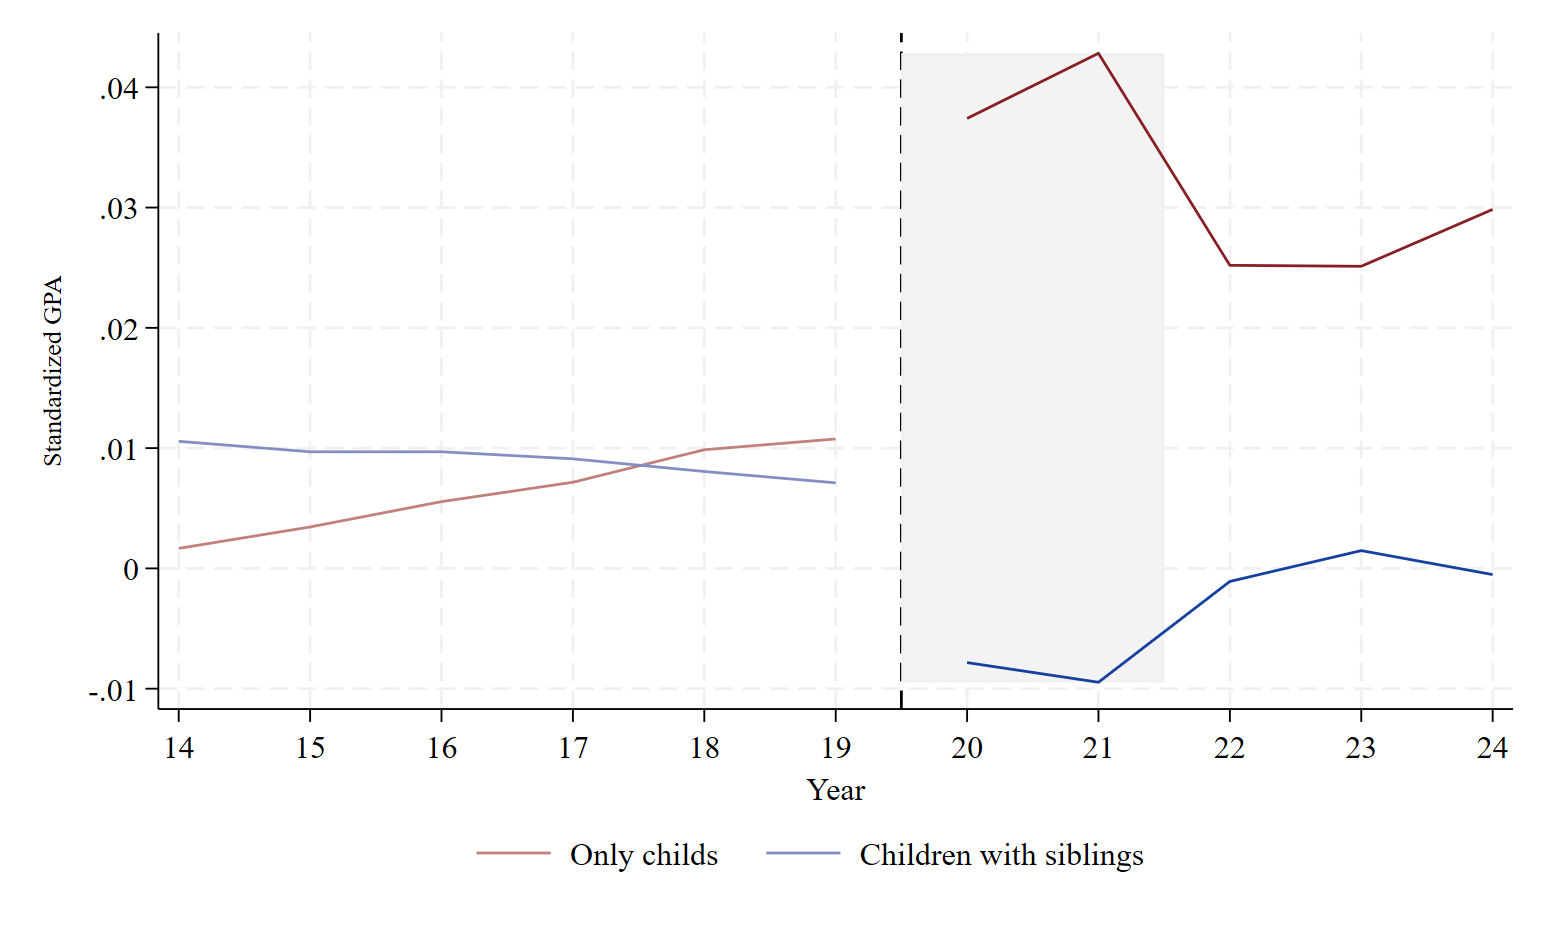
\includegraphics{./FIGURES/COVID/selected/raw_total_std_gpa_m.png}
    }
  }  
\end{frame}


\begin{frame}
    \label{raw}
    \frametitle{Raw trends of math pass rate}
        {\resizebox{0.9\textwidth}{!}{
       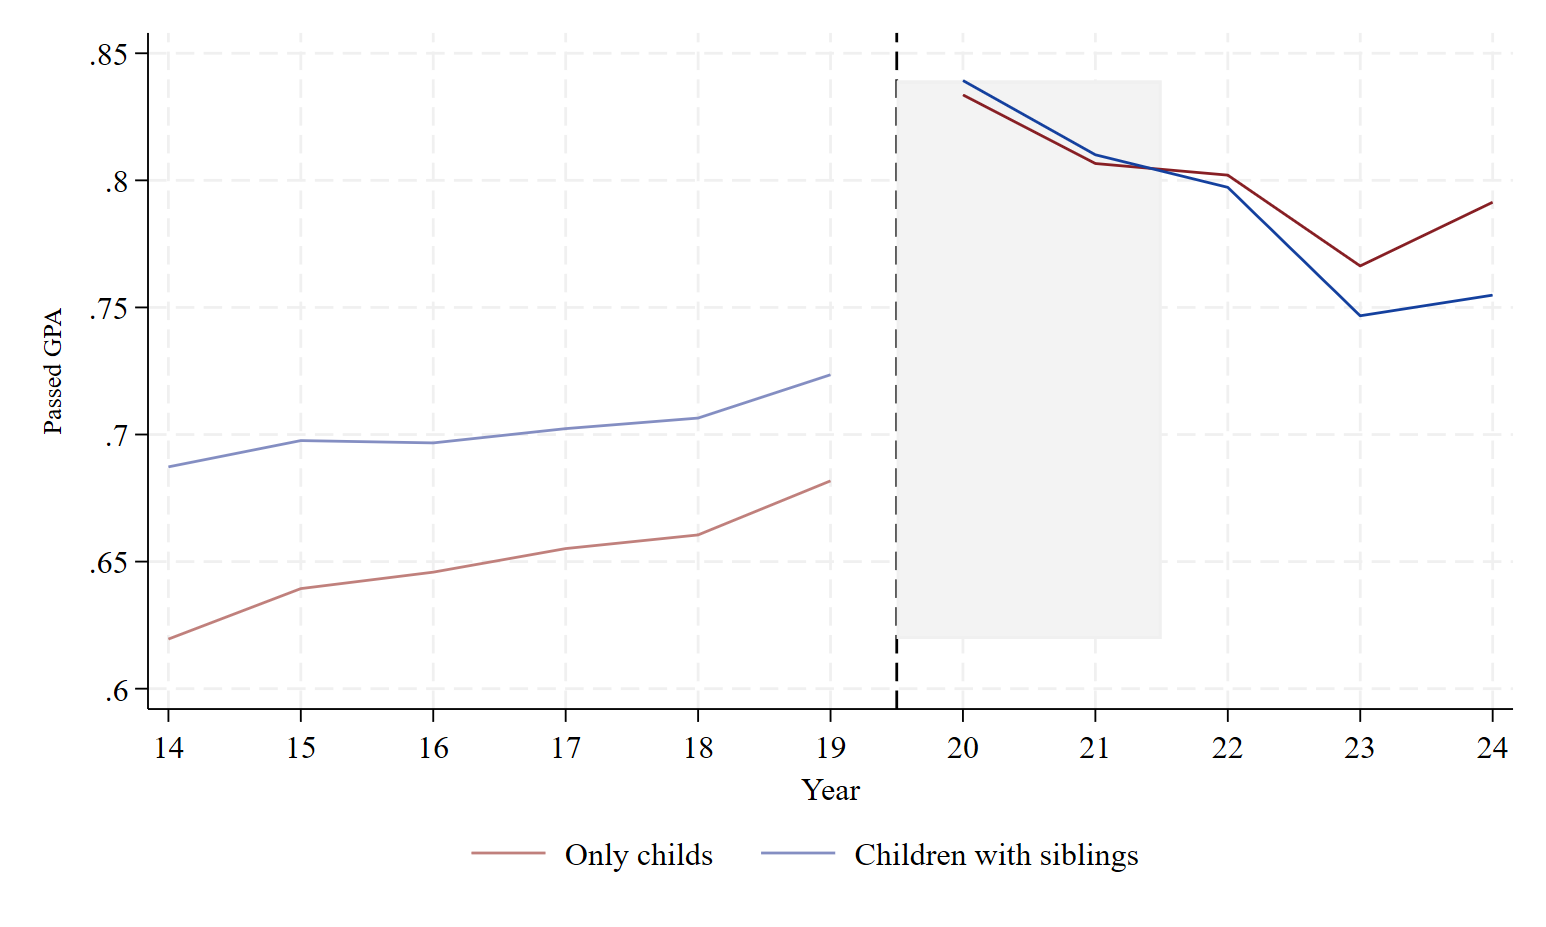
\includegraphics{./FIGURES/COVID/selected/raw_total_pass_math.png}
    }
  }  
\end{frame}

\begin{frame}
    \label{raw}
    \frametitle{Across all cohorts}
        {\resizebox{0.9\textwidth}{!}{
       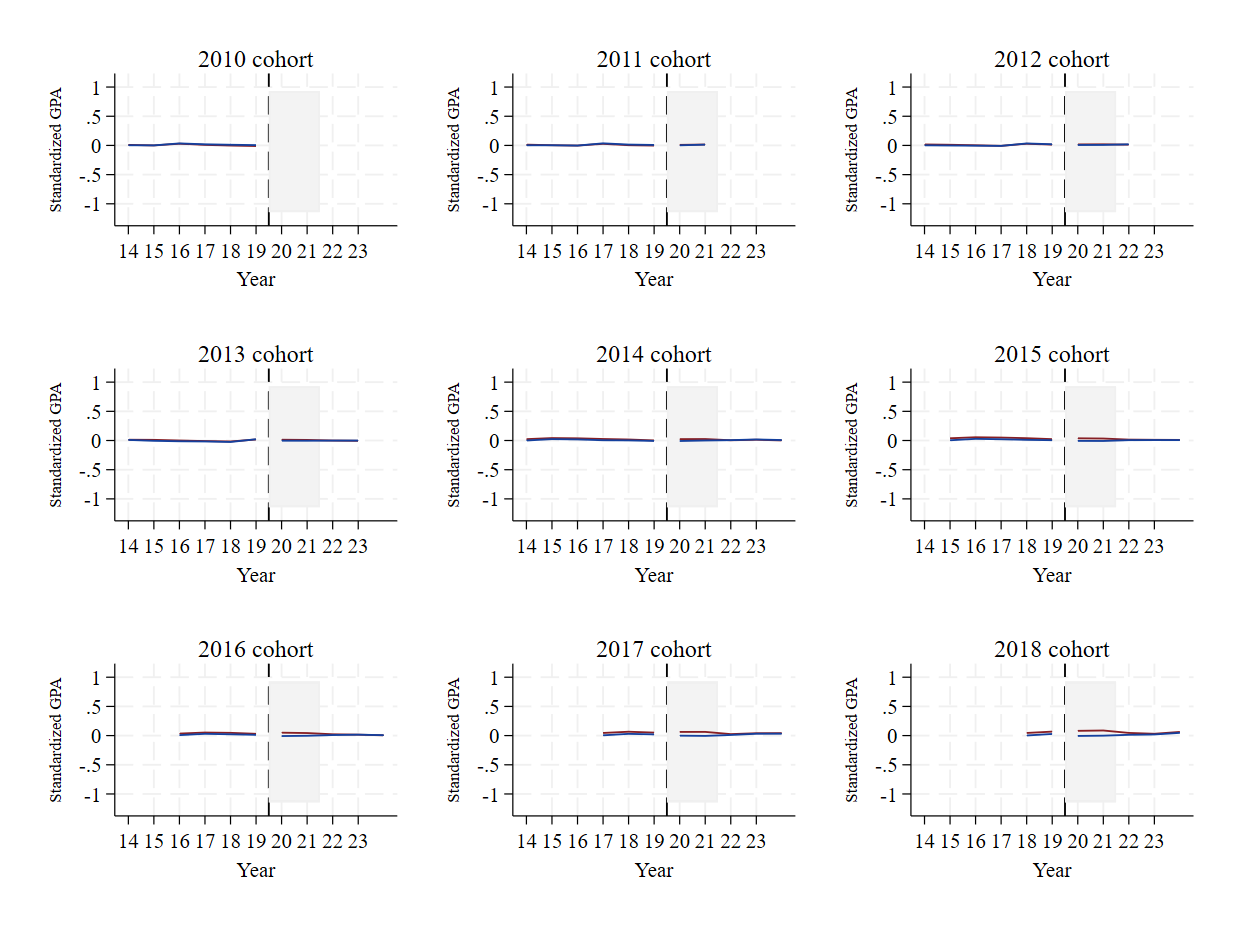
\includegraphics{./FIGURES/COVID/selected/raw_cohorts_std_gpa_m.png}
    }
  }  
\end{frame}



\begin{frame}
    \label{raw}
    \frametitle{Children with siblings do worse across different subsamples}
        {\resizebox{0.9\textwidth}{!}{
       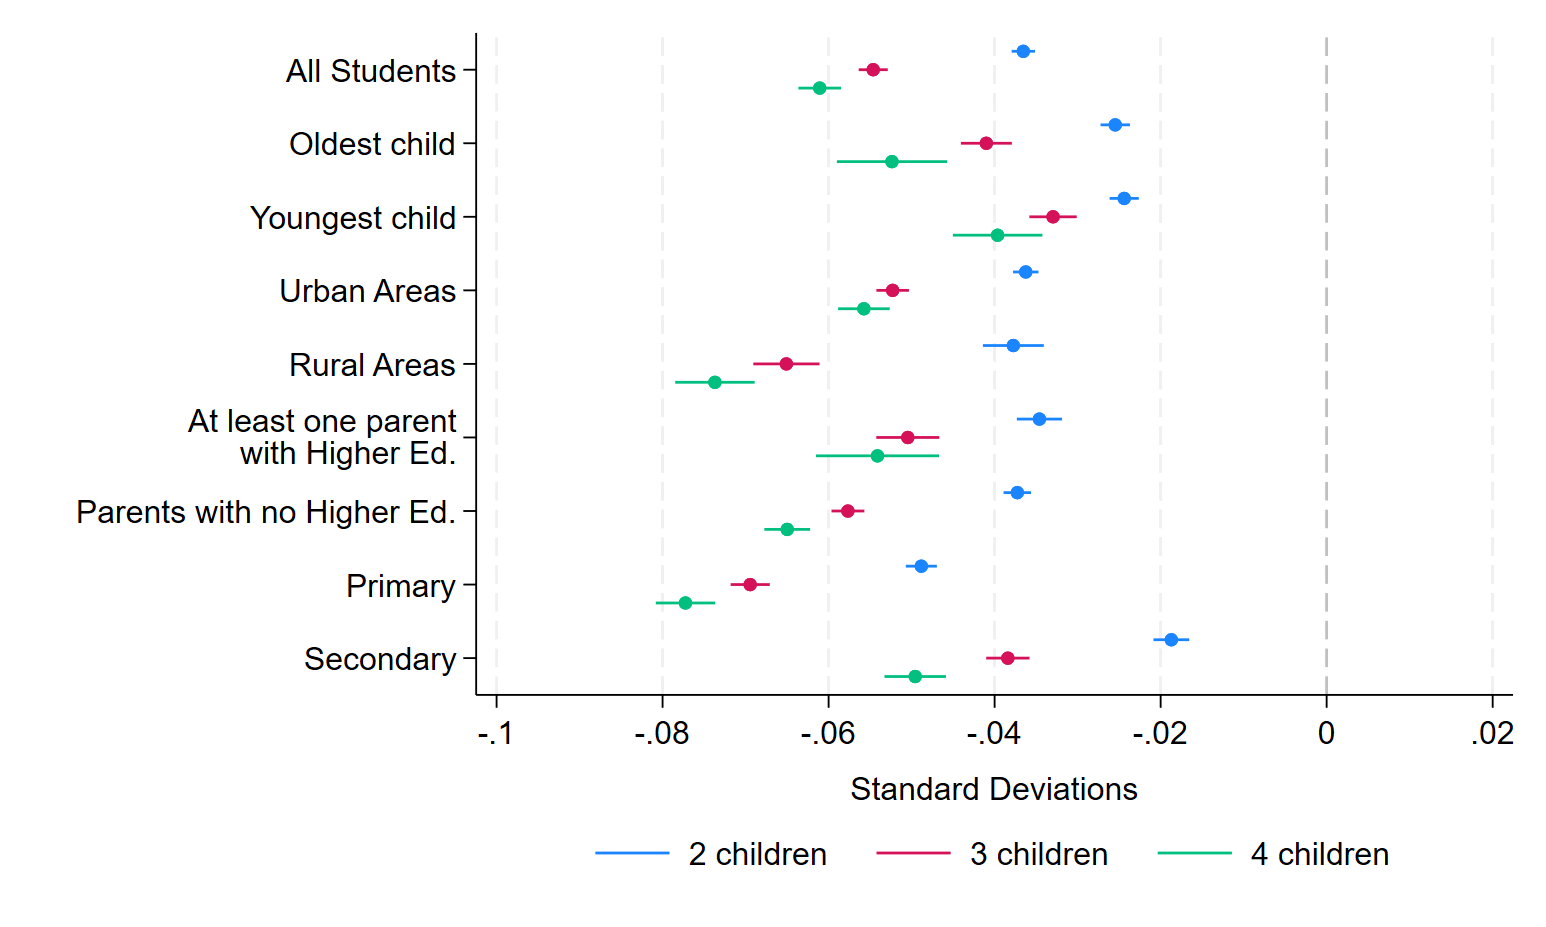
\includegraphics{./FIGURES/COVID/selected/covid_twfe_all_gpa_m_4.png}
    }
  }  
\end{frame}


\begin{frame}
    \label{raw}
    \frametitle{Resources in the household}
        {\resizebox{0.9\textwidth}{!}{
       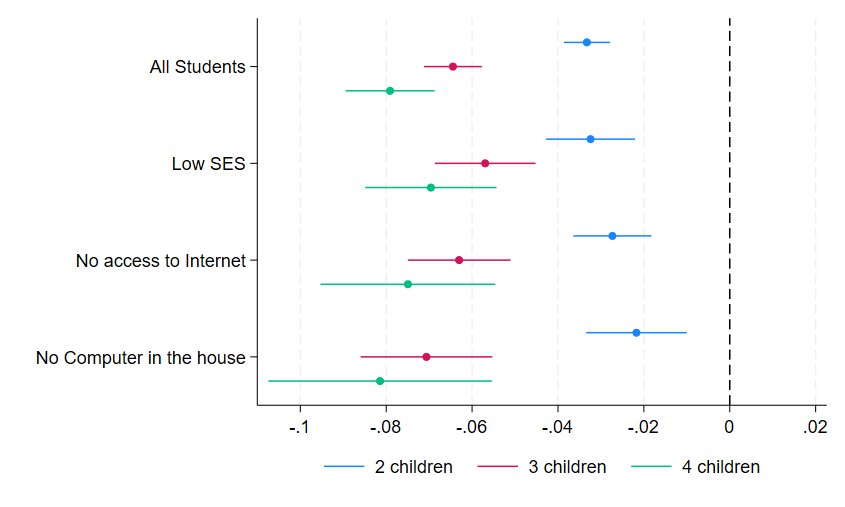
\includegraphics{./FIGURES/COVID/selected/covid_twfe_survey_elm_m_4.png}
    }
  }  
\end{frame}



\begin{frame}
    \label{raw}
    \frametitle{Event study}
        {\resizebox{0.9\textwidth}{!}{
       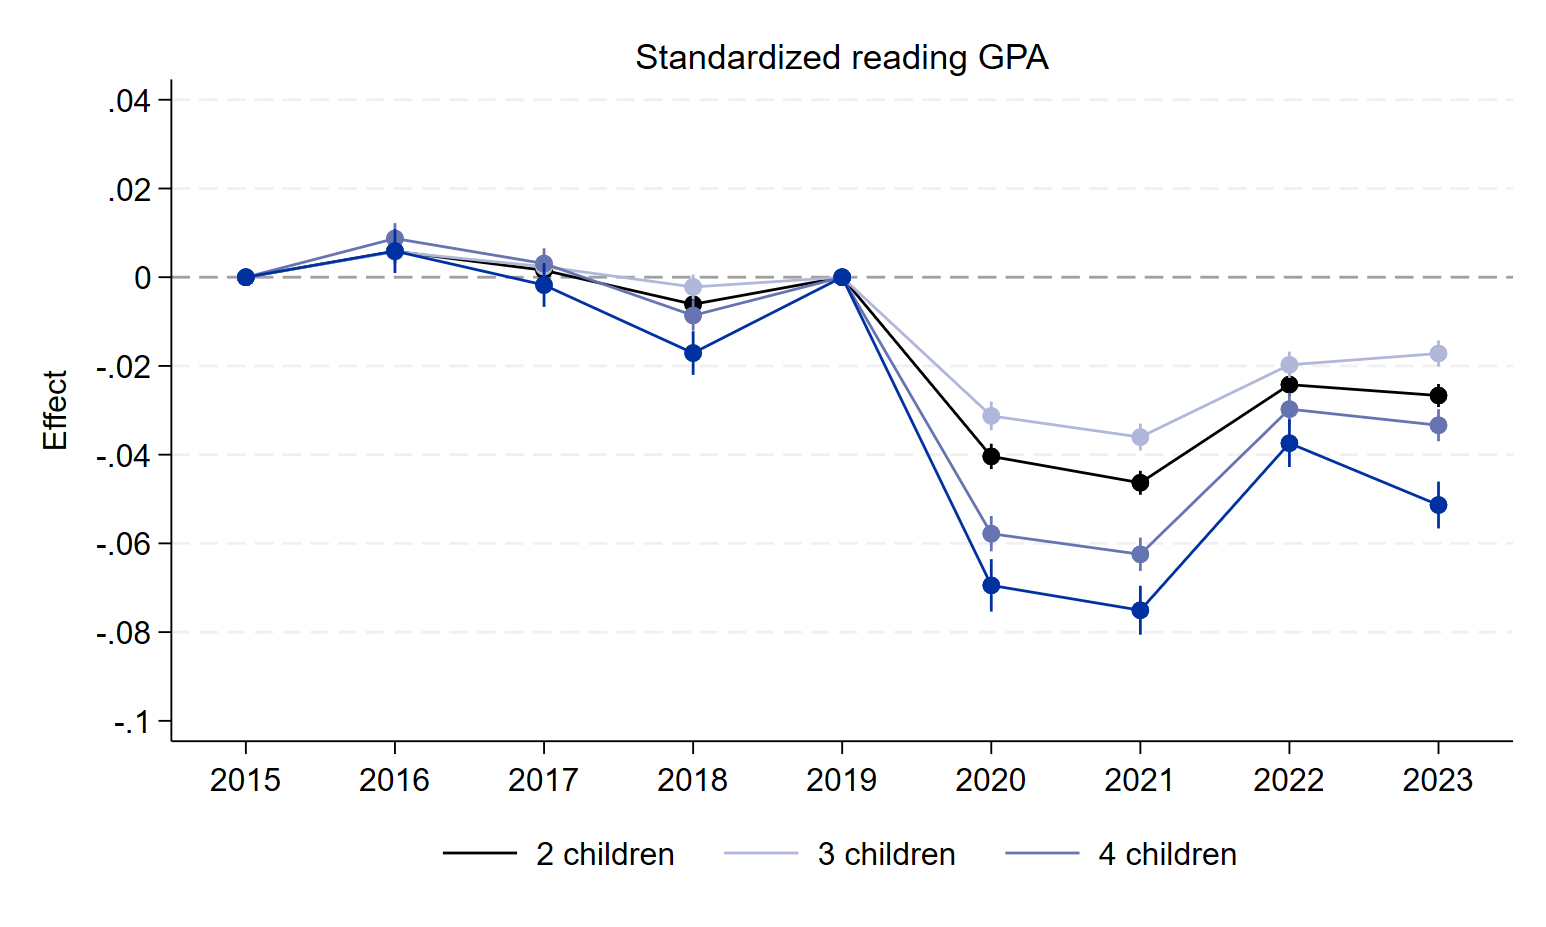
\includegraphics{./FIGURES/COVID/selected/covid_gpa_c_all_all_all_all.png}
    }
  }  
\end{frame}




\begin{frame}
    \label{event_cohort_m}
    \frametitle{Effects are slightly larger for younger cohorts}
        {\resizebox{0.9\textwidth}{!}{
       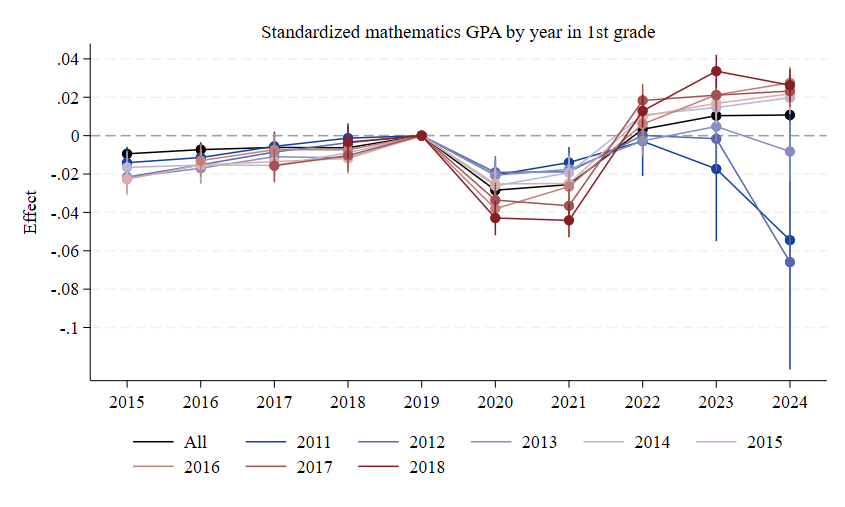
\includegraphics{./FIGURES/COVID/selected/covid_cohort_all_all_std_gpa_m.png}
    }
  }  
\end{frame}

\begin{frame}
    \label{event_cohort_m}
    \frametitle{No effect on demographics - Parent's with higher educ}
        {\resizebox{0.9\textwidth}{!}{
       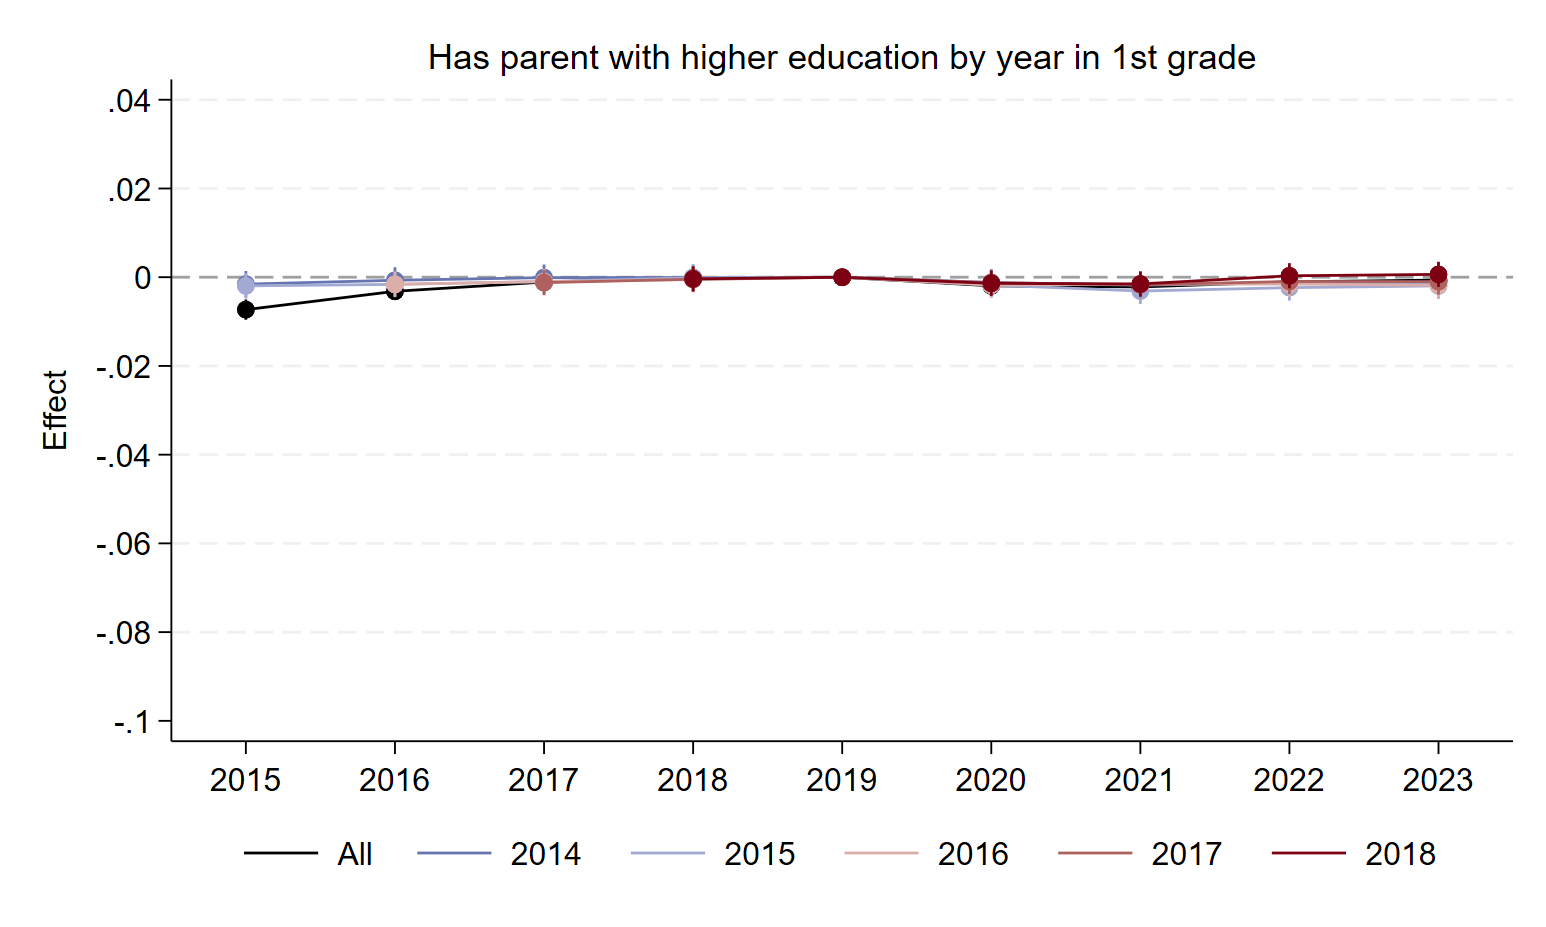
\includegraphics{./FIGURES/COVID/selected/covid_cohort_all_all_higher_ed_parent.png}
    }
  }  
\end{frame}



\begin{frame}
    \frametitle{Conclusions and next steps}
    \begin{itemize}
        \item Effects look consistent but need to be more careful with balanced panels.
        \item Will look at standardized exams taken for same grade.
        \item Can grading be the issue? Online exams + homework? So no decrease in ability but on exam performance.
        \item Look at college application exams?
    \end{itemize}
\end{frame}

\begin{frame}
    \label{event_cohort_m}
    \frametitle{Caution with TWFE by cohort}
        {\resizebox{0.9\textwidth}{!}{
       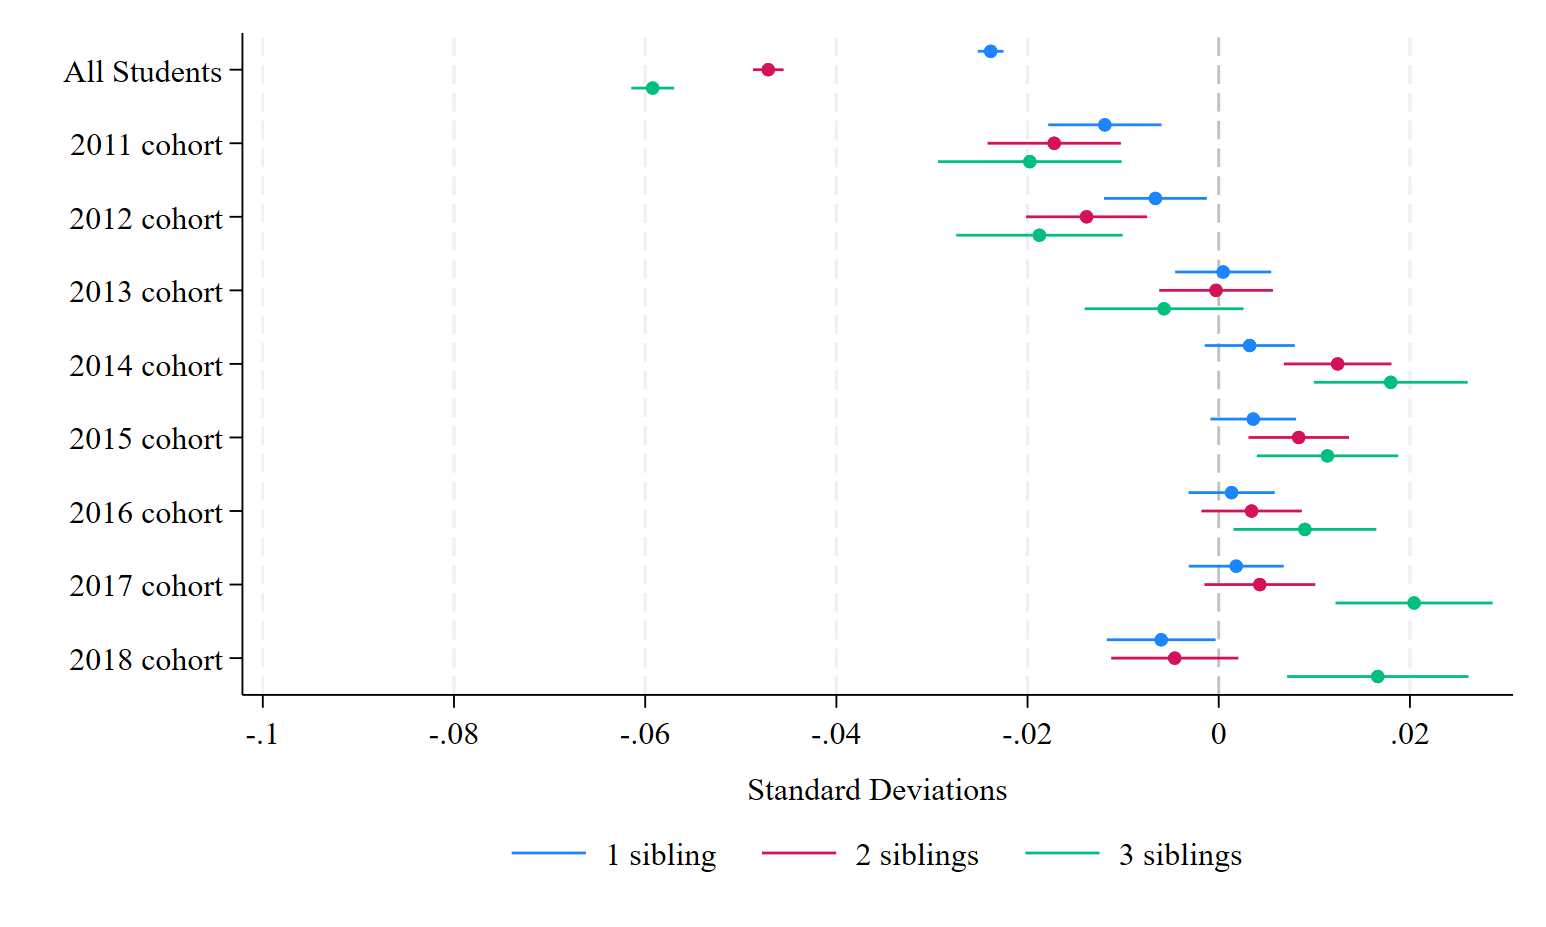
\includegraphics{./FIGURES/COVID/selected/covid_twfe_cohort_gpa_m_4.png}
    }
  }  
\end{frame}

\begin{frame}
    \label{event_cohort_m}
    \frametitle{Other literature}
    \begin{itemize}
        \item Studies heterogeneity by SES, single parents, # of siblings (1-2, vs 3+). Find effects on the first, not on # of siblings.
        \item Look at learning growth across different cohorts
   
       $\Delta Y_{ijc}= \beta Post + \epsilon_{ijc}$ 
       $\Delta Y_{ijc}= \beta Post + \gamma SES + \delta Post*SES + \epsilon_{ijc}$ 
       \item The use standardized variables with pre-mean/variance. How to replace this?
     \end{itemize}
\end{frame}

\begin{frame}
    \label{event_cohort_m}
    \frametitle{Caution with TWFE by cohort}
        {\resizebox{0.9\textwidth}{!}{
       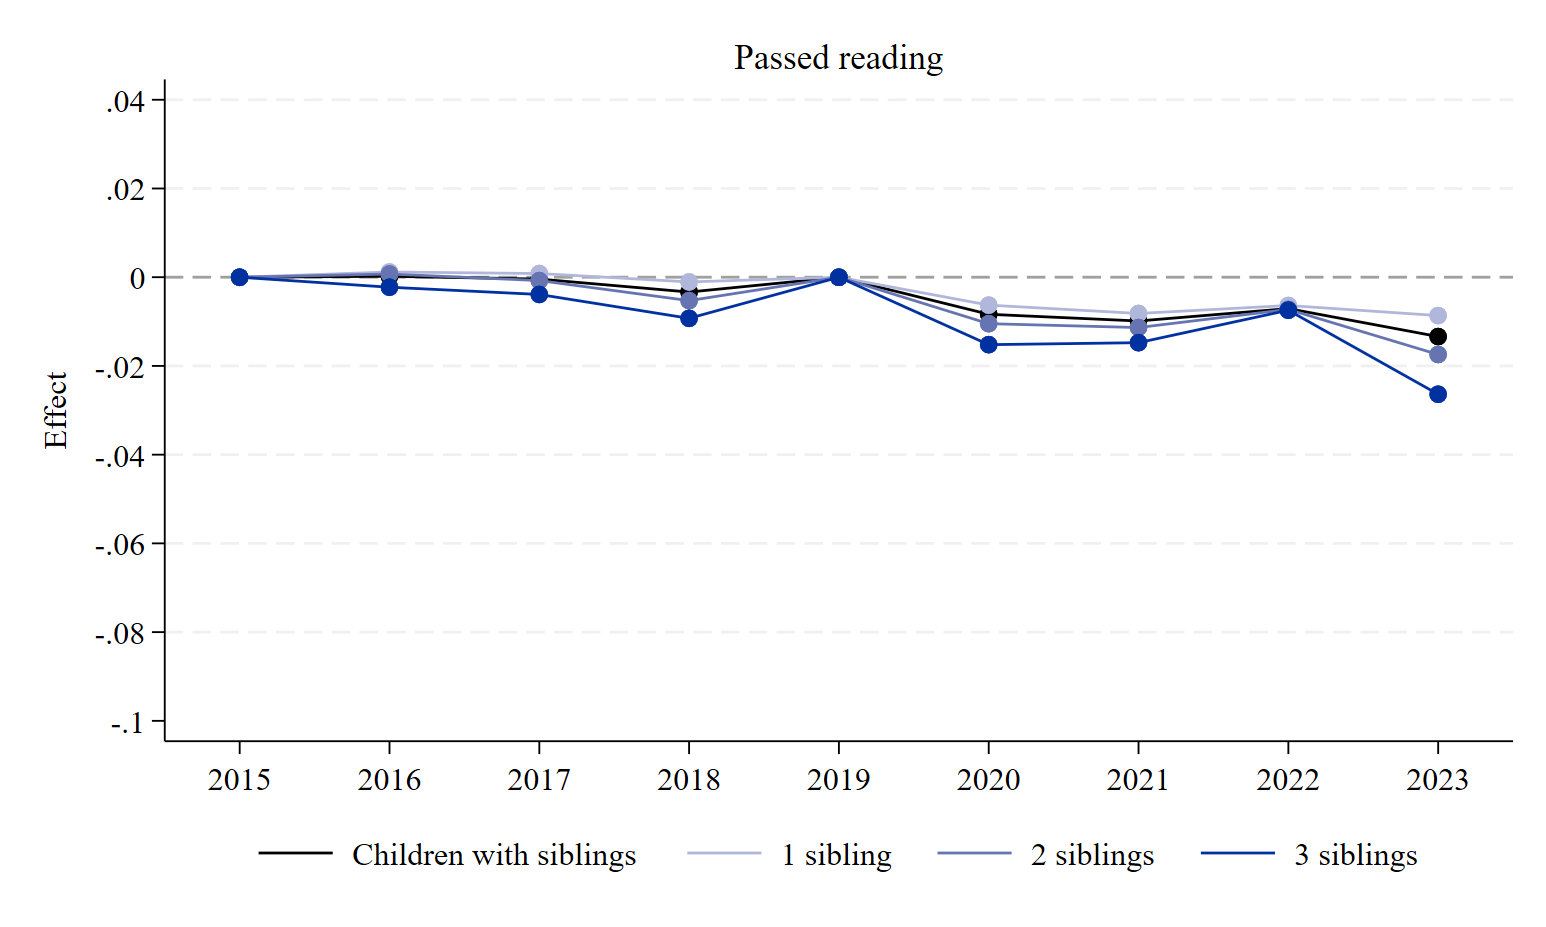
\includegraphics{./FIGURES/COVID/selected/covid_pass_read_all_all_all_elm_all.png}
    }
  }  
\end{frame}


\begin{frame}
    \label{event_cohort_m}
    \frametitle{Caution with TWFE by cohort}
        {\resizebox{0.9\textwidth}{!}{
       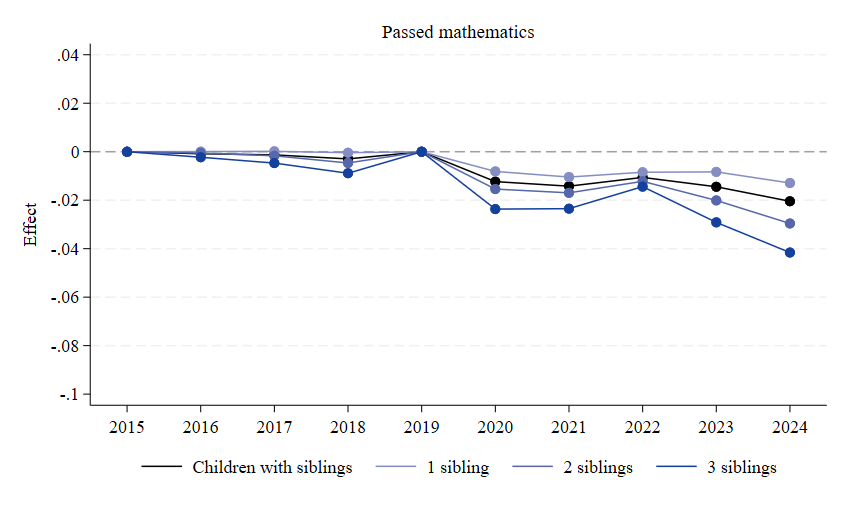
\includegraphics{./FIGURES/COVID/selected/covid_pass_math_all_all_all_elm_all.png}
    }
  }  
\end{frame}

\begin{frame}
    \label{update_scott}
    \frametitle{Some updates}
    \begin{itemize}
        \item Advancing to candidacy
        \item Raw plots for each grade
        \item Single parents or `lives with parents
        \item Is the bounce back a recovery or new kids coming in?
        \item Larry Kenny
        \item Evidence from Netherlands
        \item Grade thresholds and Distribution
    \end{itemize}
\end{frame}


\begin{frame}
    \label{update_scott}
    \frametitle{GPAs across cohorts and across grades}
    \begin{itemize}
        \item Last time I showed results by cohort over time.
        \item Now I show results of grades over time
    \end{itemize}
\end{frame}


\begin{frame}
    \label{update_scott}
    \frametitle{Raw plots per cohort - Age trend}
        {\resizebox{0.9\textwidth}{!}{
       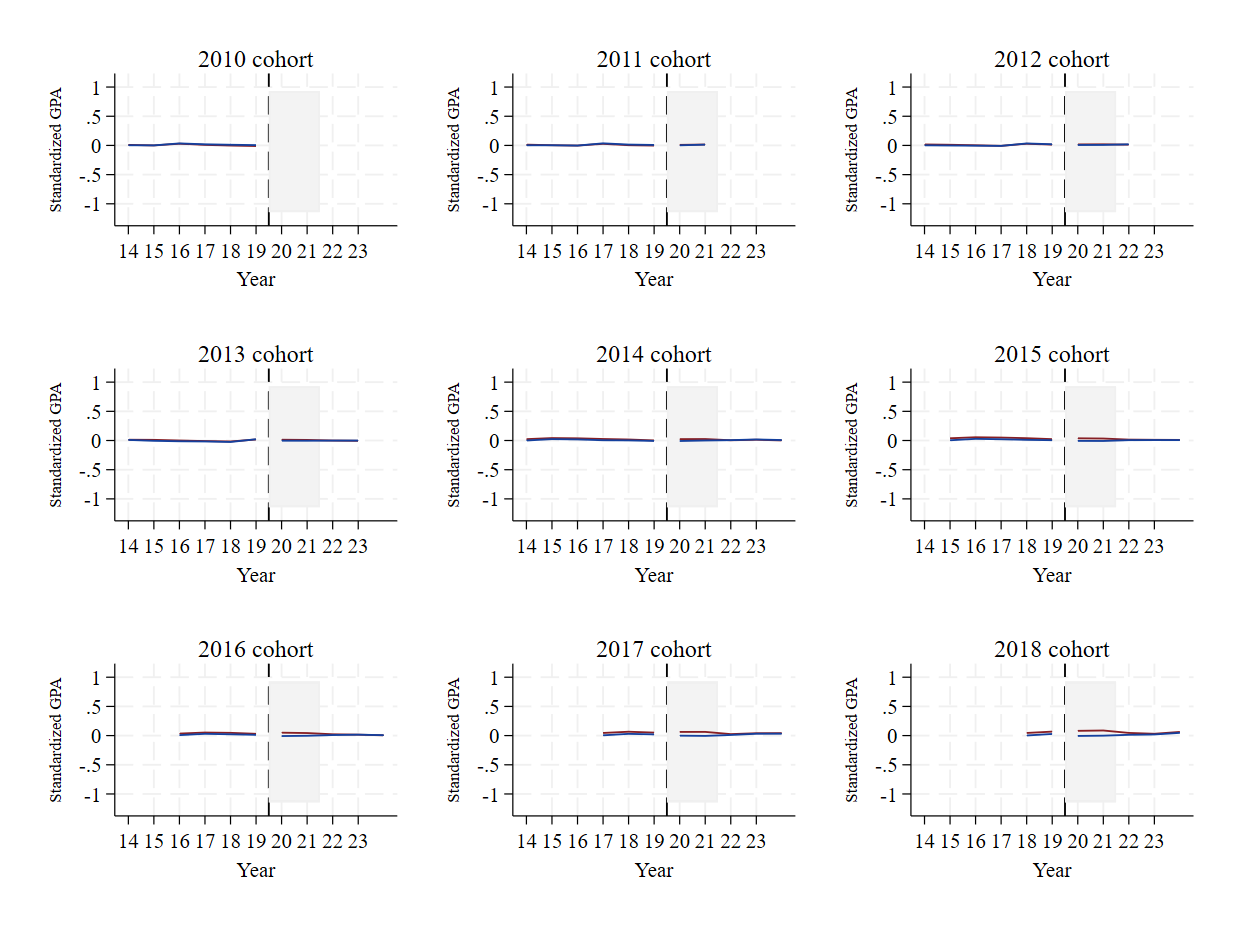
\includegraphics{./FIGURES/COVID/selected/raw_cohorts_std_gpa_m.png}
      }
    }
\end{frame}

\begin{frame}
    \label{update_scott}
    \frametitle{Raw plots per grade - Time trend}
        {\resizebox{0.8\textwidth}{!}{
       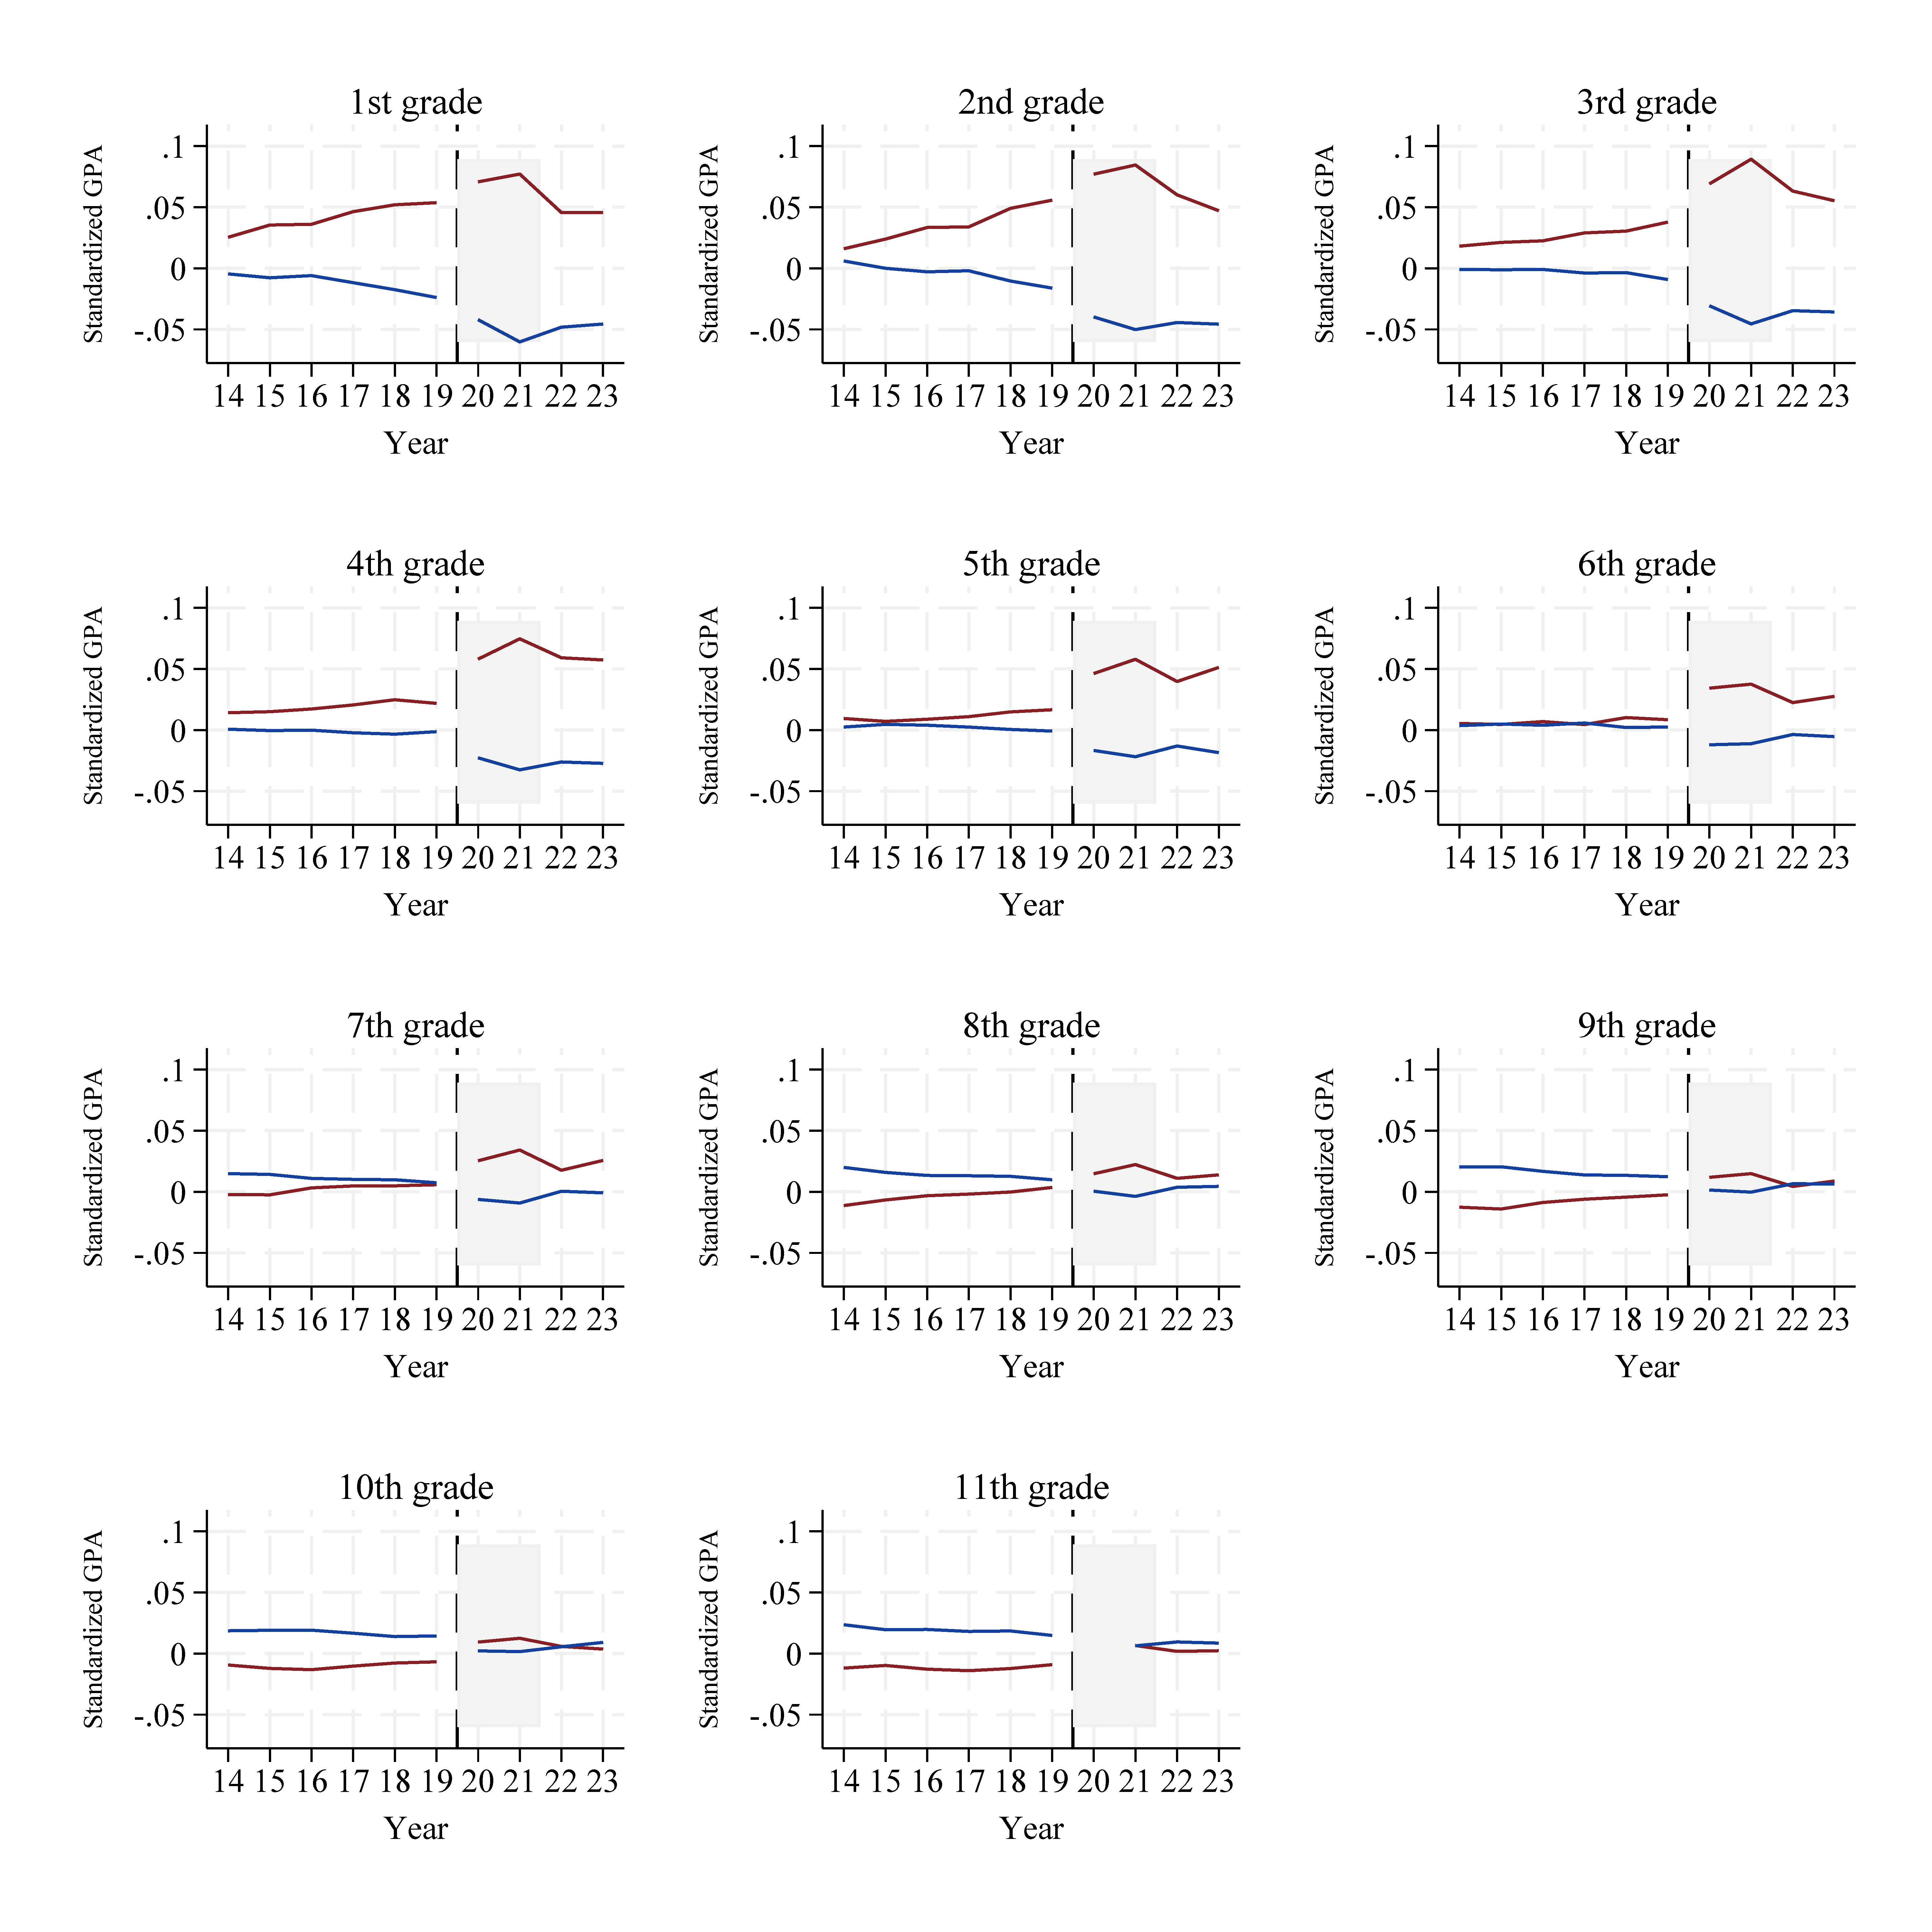
\includegraphics{./FIGURES/COVID/selected/raw_grades_std_gpa_m.pdf}
      }
    }
\end{frame}

\begin{frame}
    \label{update_scott}
    \frametitle{Single parents}
        {\resizebox{0.9\textwidth}{!}{
       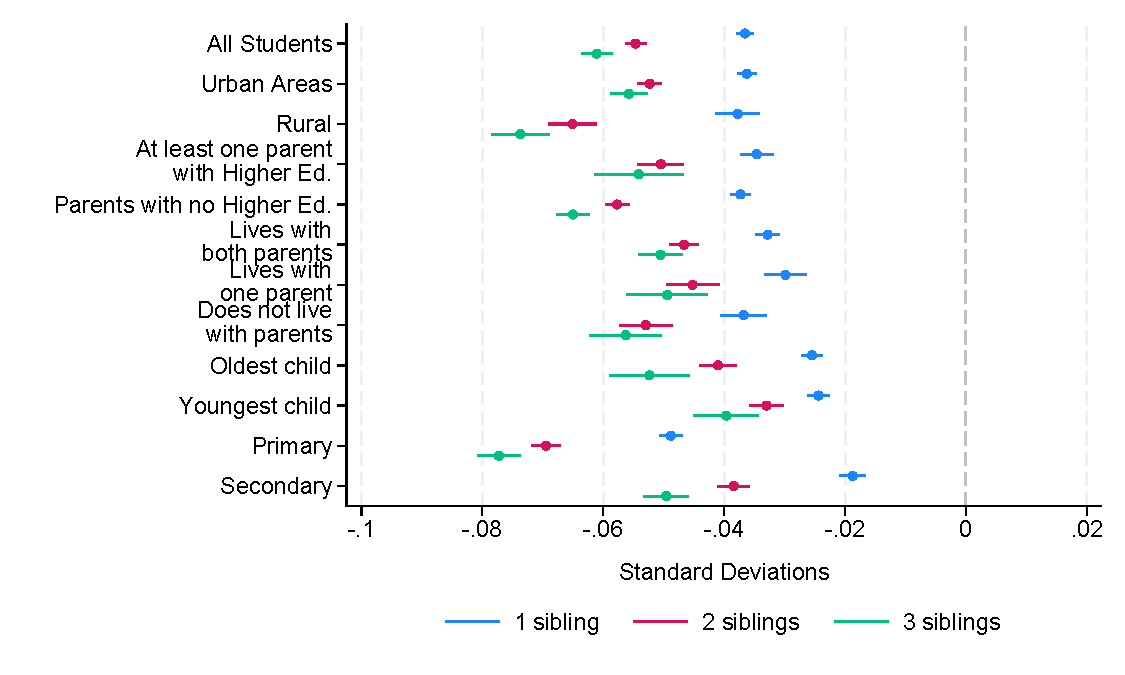
\includegraphics{./FIGURES/COVID/selected/covid_twfe_all_gpa_m_4.pdf}
      }
    }
\end{frame}

\begin{frame}
    \label{update_scott}
    \frametitle{Bounce back and standardized exams}
    \begin{itemize}
        \item I've been looking at within school-grade GPA.
        \item I now look at Standardized national examinations. 
        \begin{itemize}
            \item Better to address overall learning losses (not just relative)
            \item More accurate measure of ability.
        \end{itemize}
        \item Information is not perfect. Sometimes census, sometimes survey. Not all grades, not all years.
    \end{itemize}
\end{frame}

\begin{frame}
    \label{update_scott}
    \frametitle{2nd grade}
        {\resizebox{0.9\textwidth}{!}{
       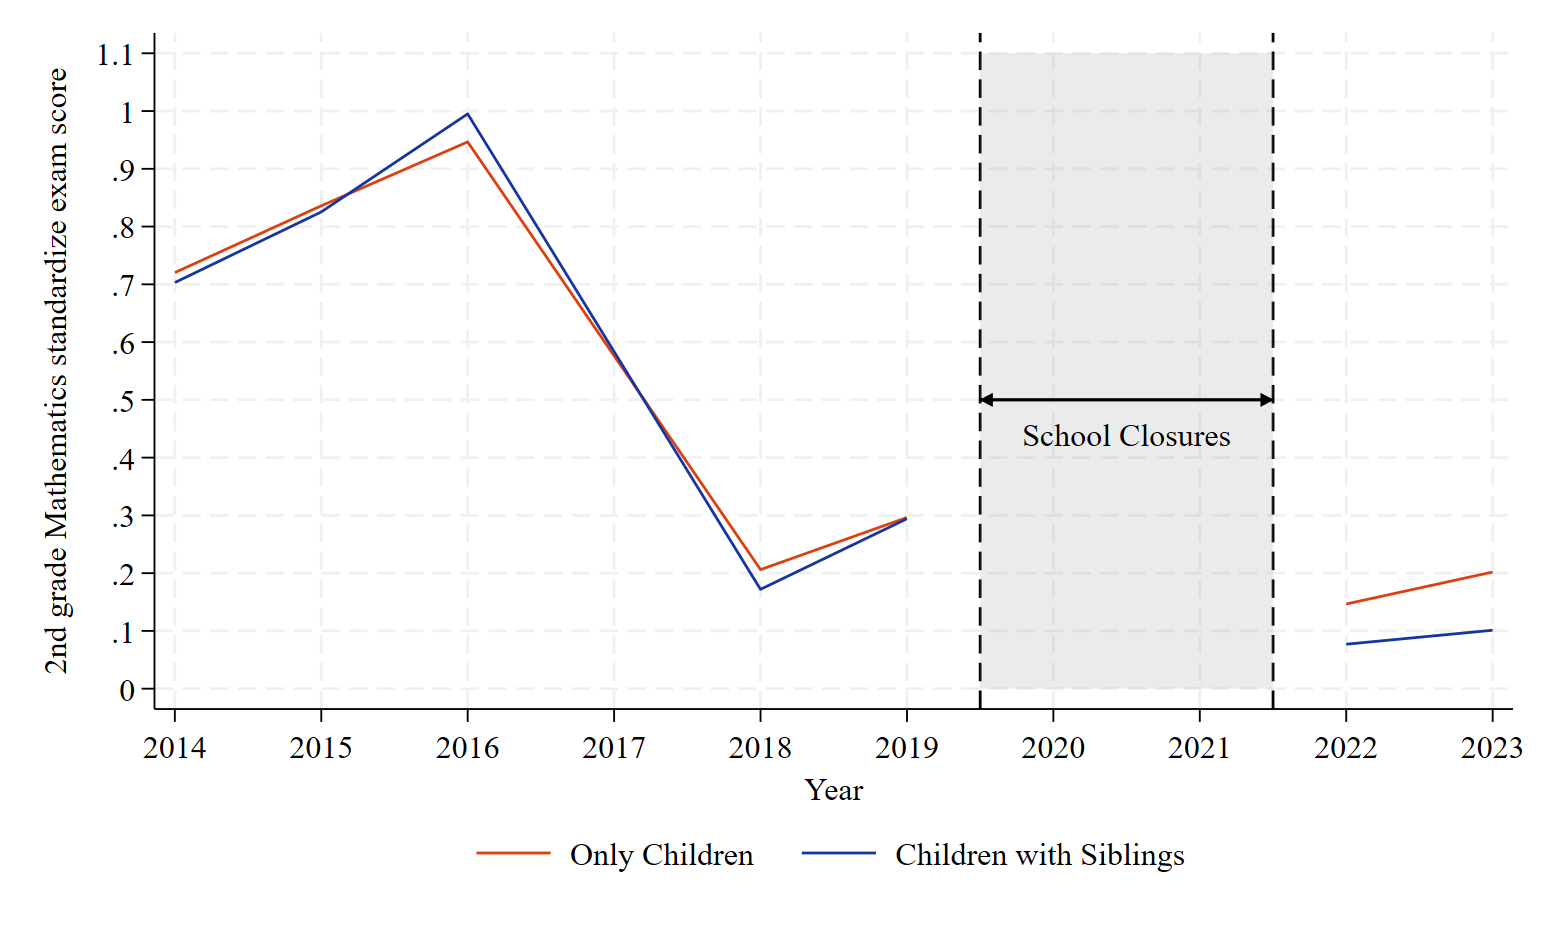
\includegraphics{./FIGURES/COVID/selected/raw_ece_math_2.png}
      }
    }
\end{frame}

\begin{frame}
    \label{update_scott}
    \frametitle{4th grade}
        {\resizebox{0.9\textwidth}{!}{
       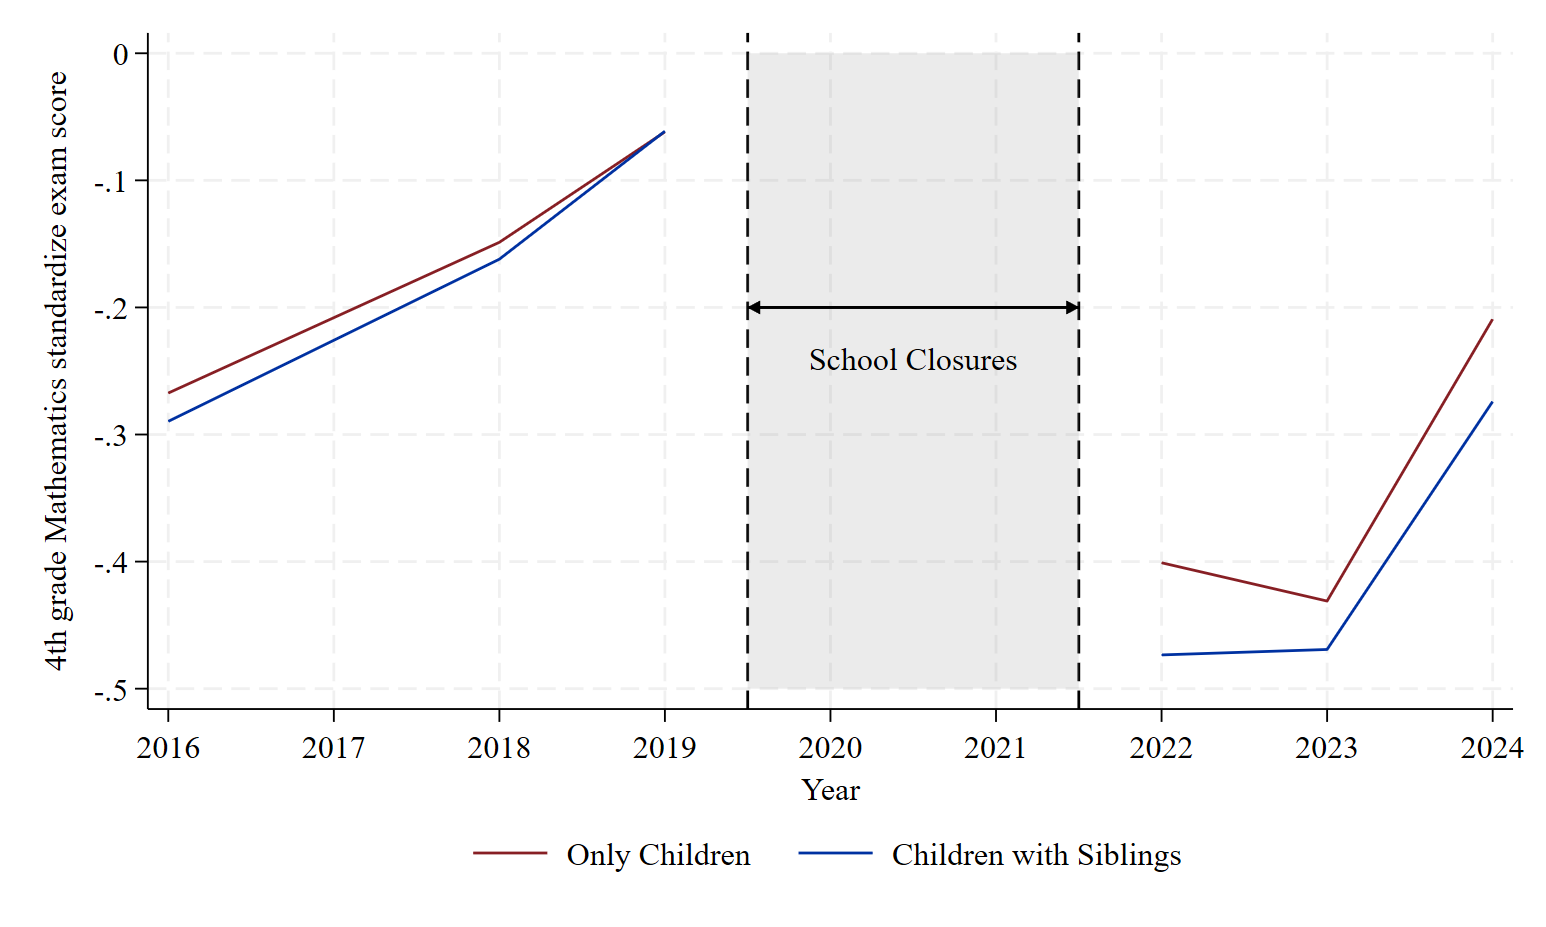
\includegraphics{./FIGURES/COVID/selected/raw_ece_math_4.png}
      }
    }
\end{frame}

\begin{frame}
    \label{update_scott}
    \frametitle{8th grade}
        {\resizebox{0.9\textwidth}{!}{
       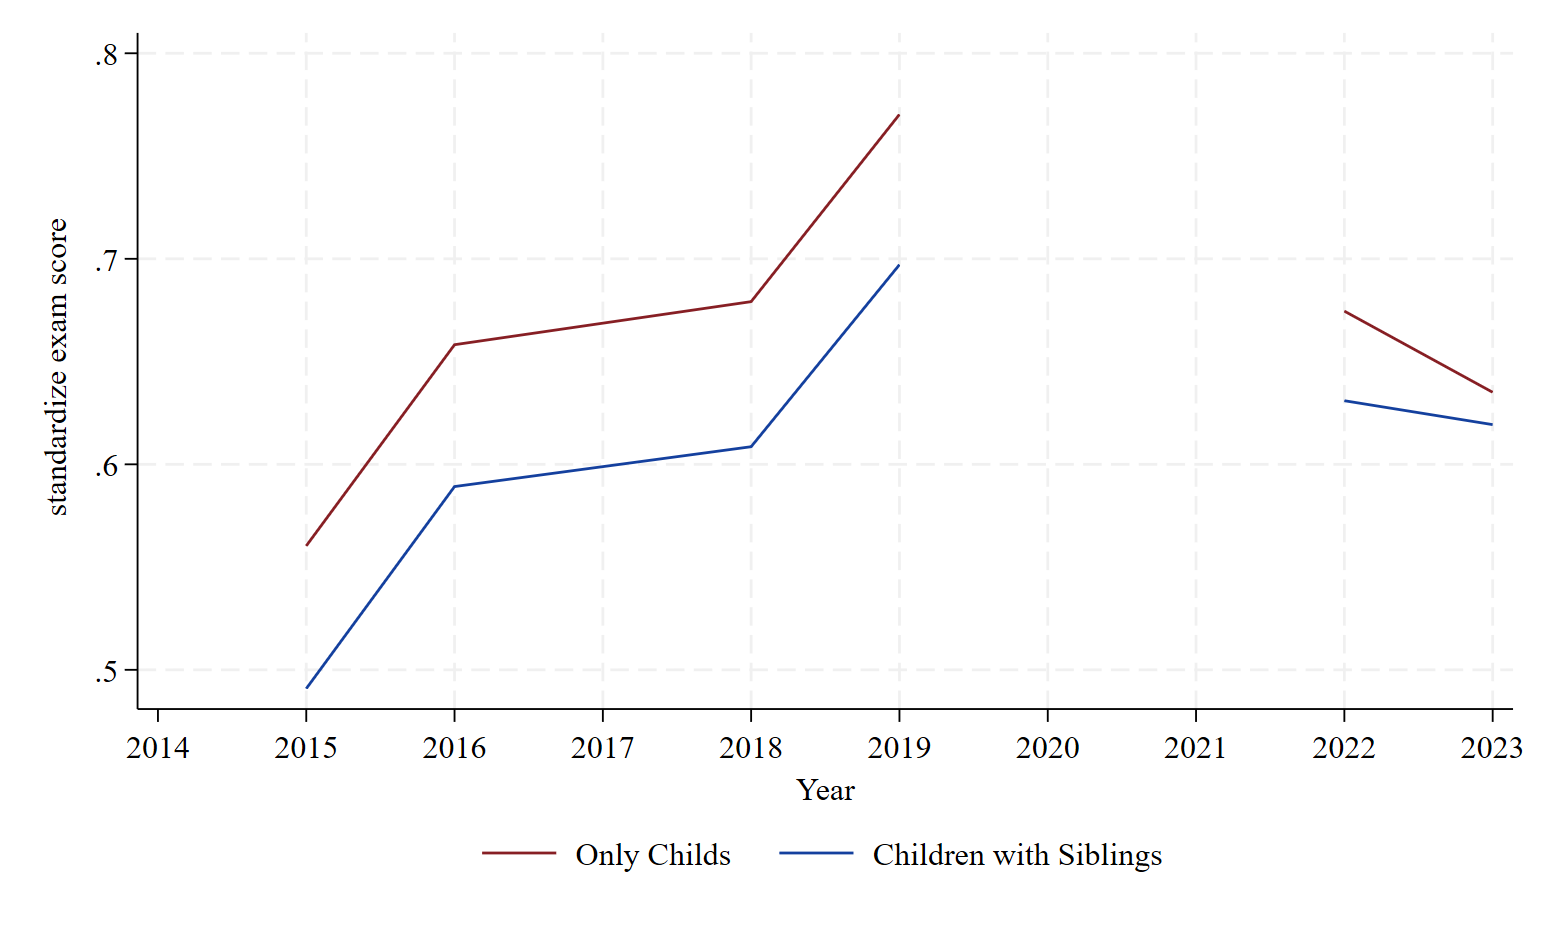
\includegraphics{./FIGURES/COVID/selected/raw_ece_math_8.png}
      }
    }
\end{frame}


\begin{frame}
    \label{update_scott}
    \frametitle{Larry Kenny}
    \begin{itemize}
        \item Check paper
        \item Inputs debate: Past and present
        \item 
    \end{itemize}
\end{frame}

\begin{frame}
    \label{event_cohort_m}
    \frametitle{Evidence from the Netherlands}
    \begin{itemize}
        \item Had 2 school closures during 1.5 years of Covid. $\approx$ 8 weeks of closure.
        \item Studies heterogeneity by SES, single parents, # of siblings (1-2, vs 3+). Find effects on the first, not on # of siblings.
        \item Look at learning growth across different cohorts
   
       $\Delta Y_{ijc}= \beta Post + \epsilon_{ijc}$ 
       $\Delta Y_{ijc}= \beta Post + \gamma SES + \delta Post*SES + \epsilon_{ijc}$ 
     \end{itemize}
\end{frame}

\begin{frame}
    \label{event_cohort_m}
    \frametitle{Doing a similar approach}
        {\resizebox{0.9\textwidth}{!}{
       %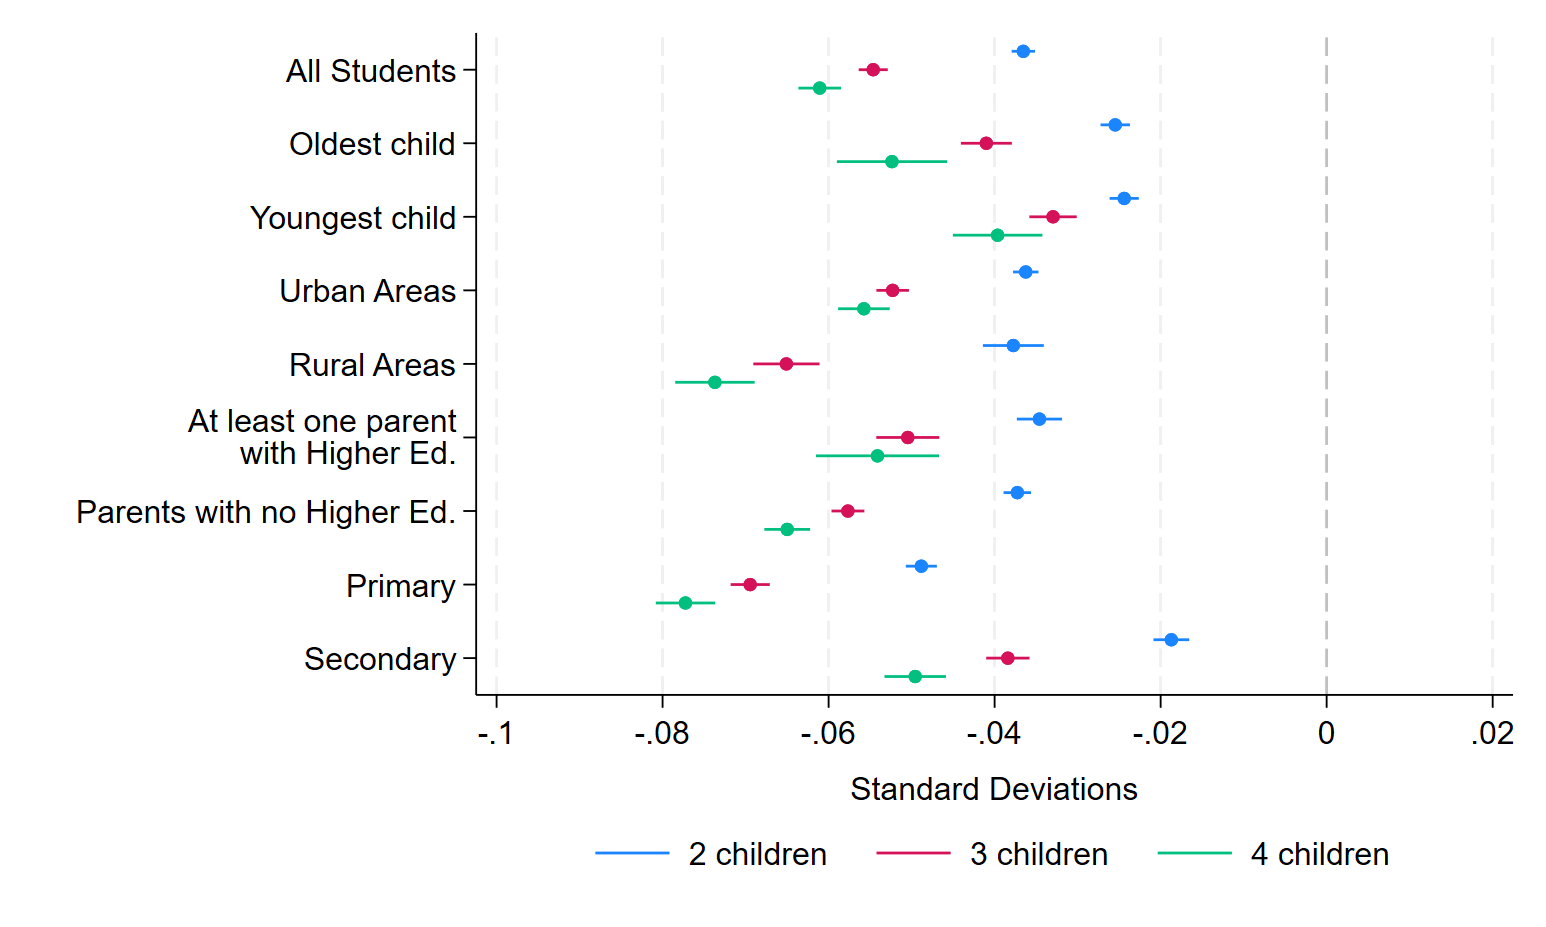
\includegraphics{./FIGURES/COVID/selected/covid_twfe_all_gpa_m_4.png}
      }
    }
\end{frame}


\begin{frame}
    \label{update_scott}
    \frametitle{Grade thresholds during covid}
    \begin{itemize}
        \item During covid (full academic year 2020 and 2021) all children were promoted and no subject was failed. 
        \item D grade was elimiated and grades went from 0-20 to 11-20.
        \item This could cause an spurious effect if one population was more likely below the passing grade
    \end{itemize}
\end{frame}


\begin{frame}
    \label{update_scott}
    \frametitle{Grade distributions pre-covid: Elementary}
 {\resizebox{0.9\textwidth}{!}{
       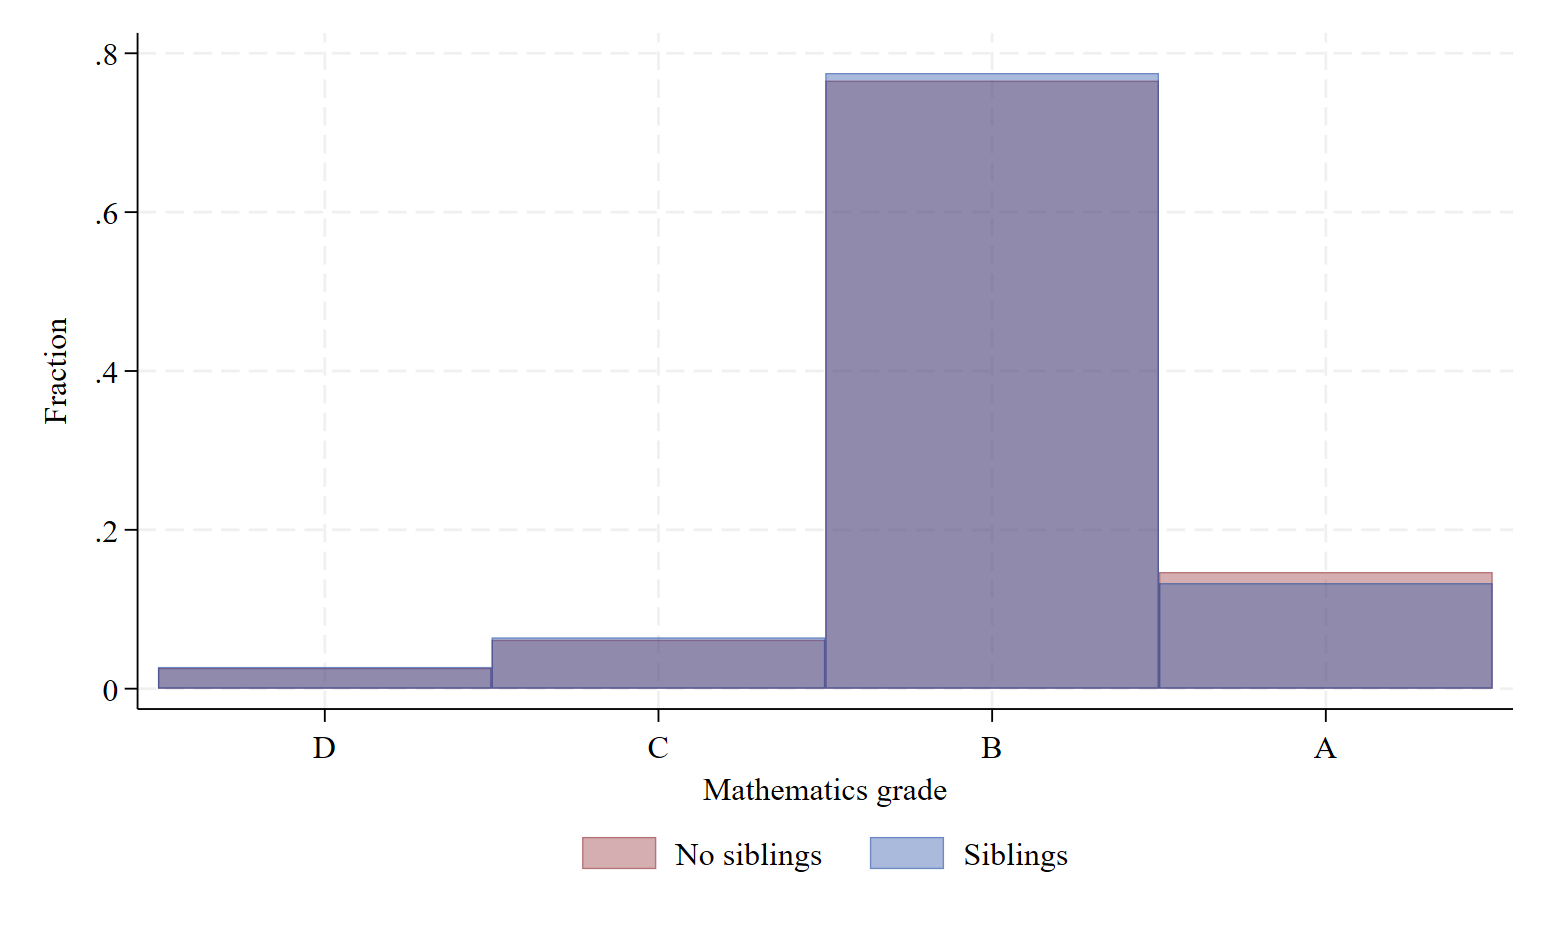
\includegraphics{./FIGURES/COVID/selected/histogram_pre_elm.png}
      }
    }
\end{frame}

\begin{frame}
    \label{update_scott}
    \frametitle{Grade distributions pre-covid: Secondary}
 {\resizebox{0.9\textwidth}{!}{
       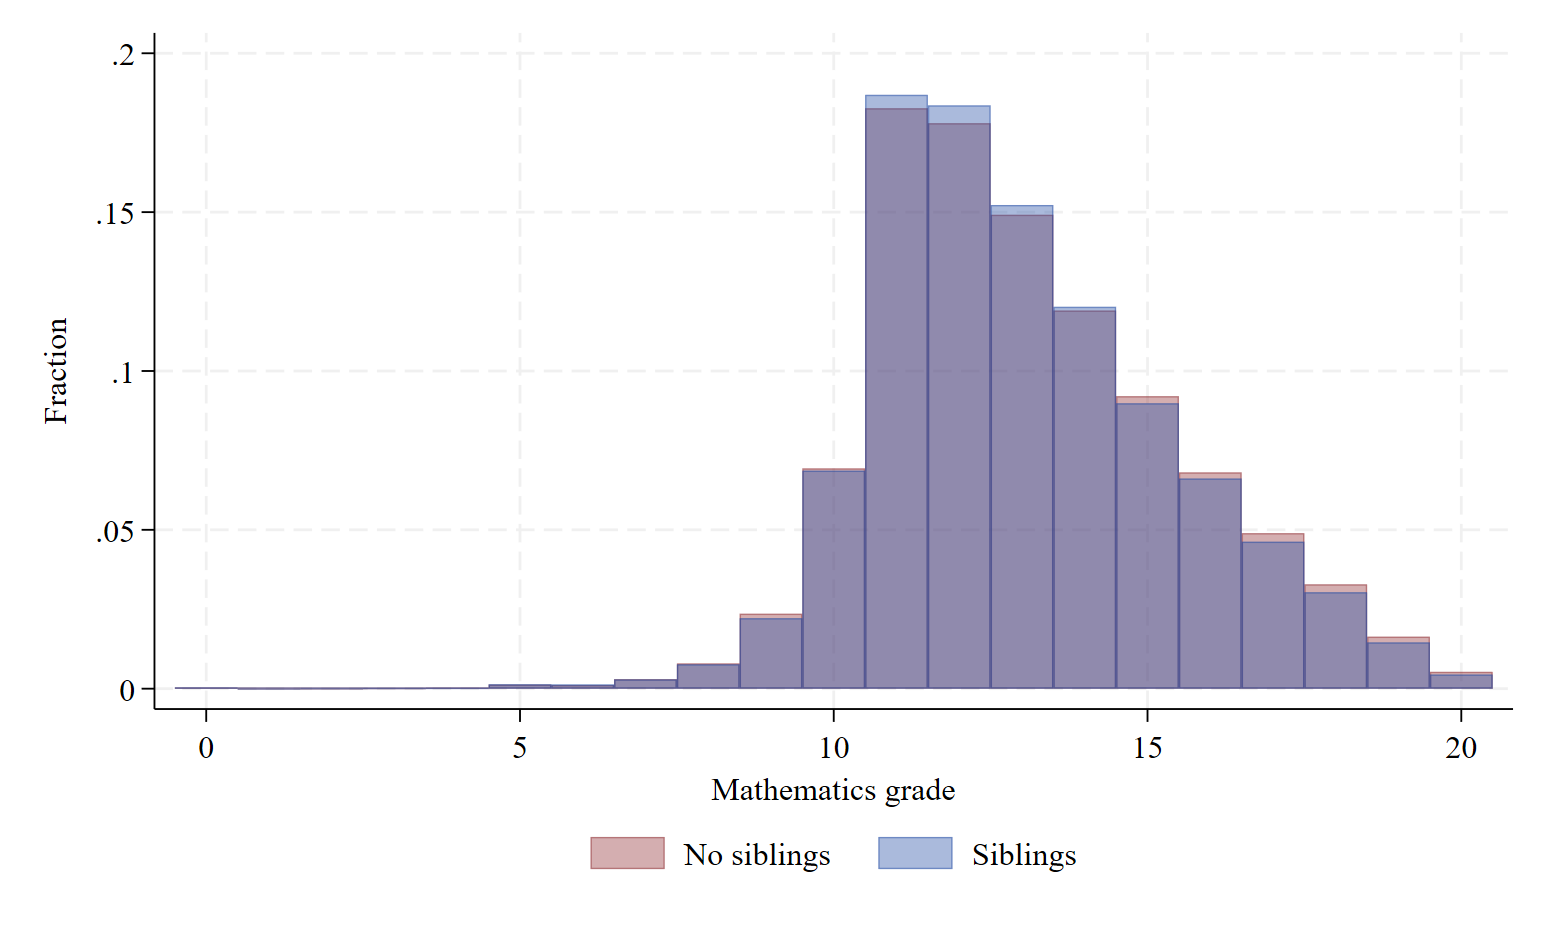
\includegraphics{./FIGURES/COVID/selected/histogram_pre_9-10.png}
      }
    }
\end{frame}

\begin{frame}
    \label{update_scott}
    \frametitle{Grade distributions post-covid: Elementary}
 {\resizebox{0.9\textwidth}{!}{
       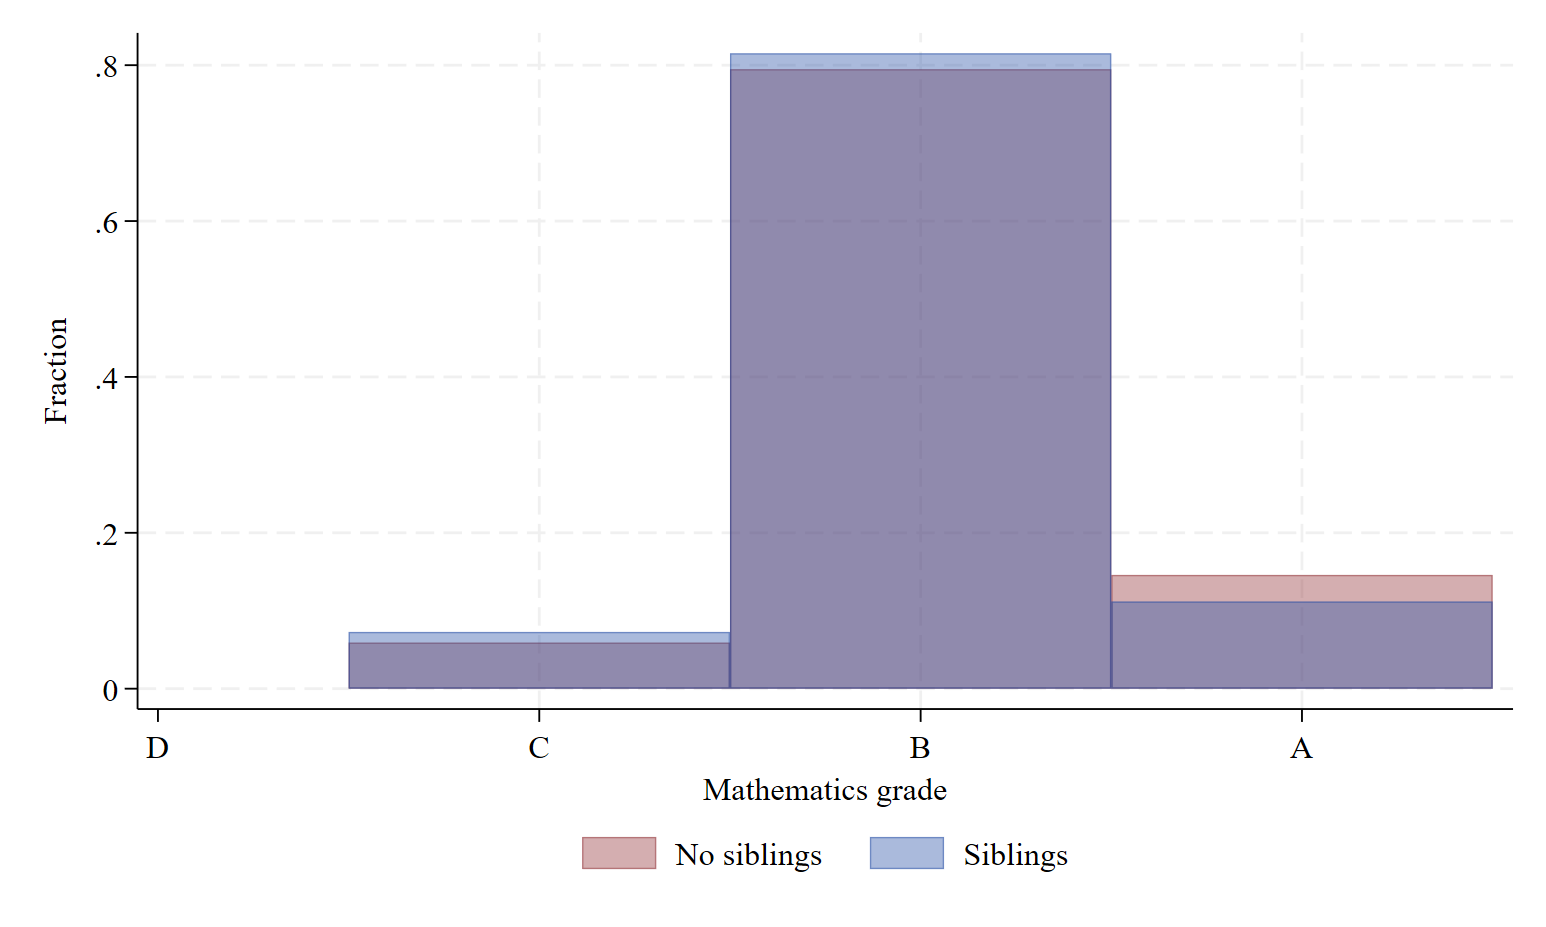
\includegraphics{./FIGURES/COVID/selected/histogram_post_elm.png}
      }
    }
\end{frame}

\begin{frame}
    \label{update_scott}
    \frametitle{Grade distributions post-covid: Secondary}
 {\resizebox{0.9\textwidth}{!}{
       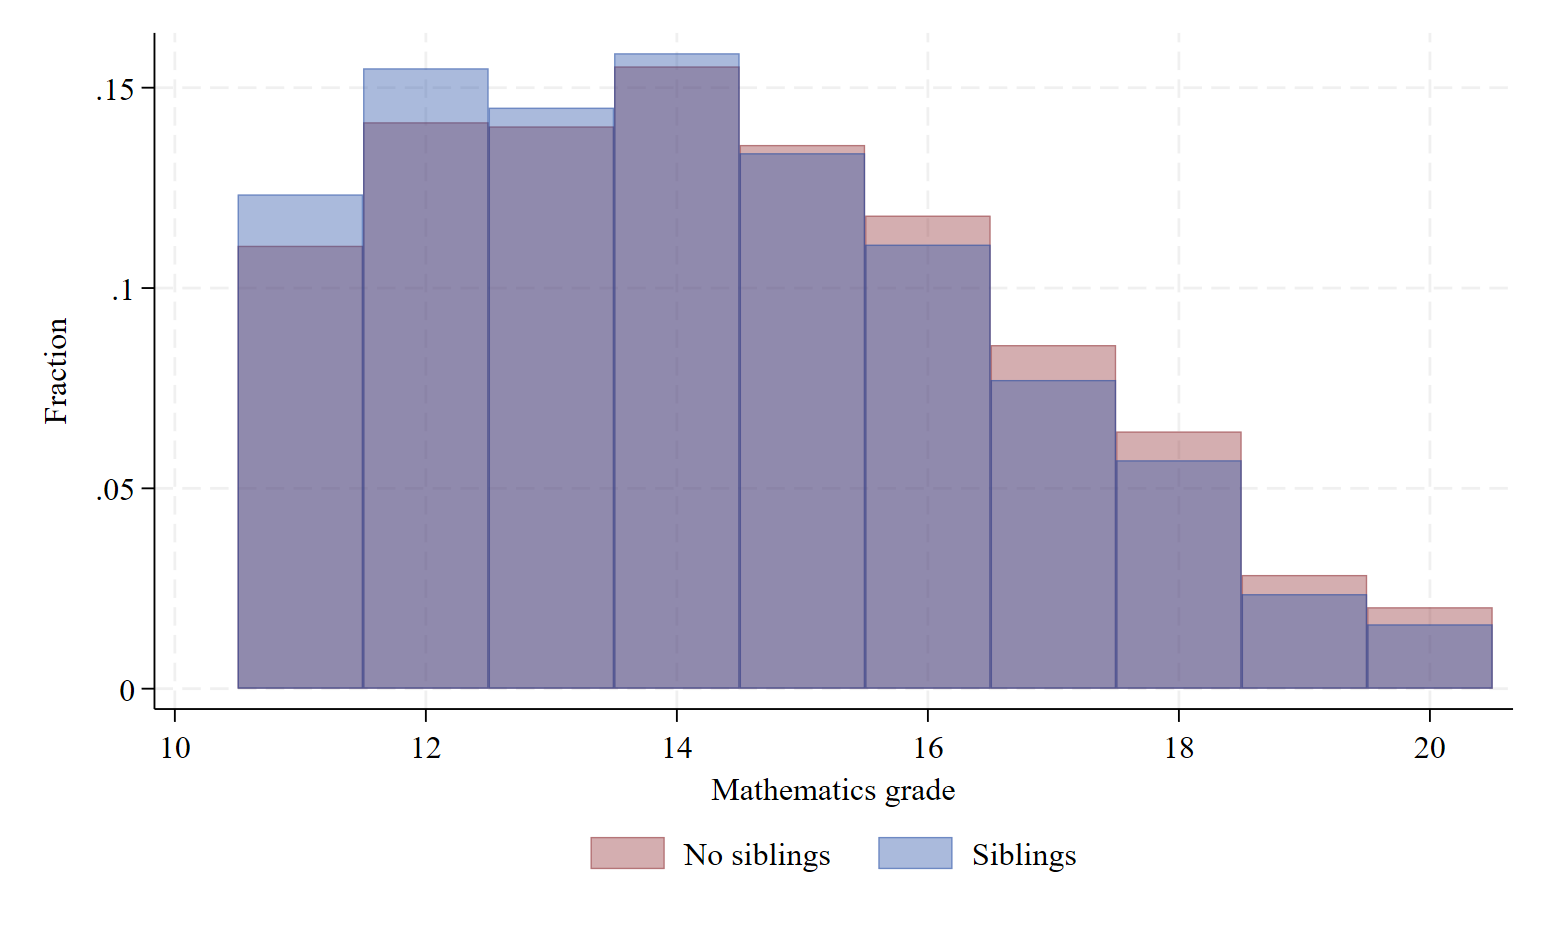
\includegraphics{./FIGURES/COVID/selected/histogram_post_9-10.png}
      }
    }
\end{frame}

\begin{frame}
    \label{update_scott}
    \frametitle{Time Use Surveys}
    \begin{itemize}
        \item 2013 and 2024. Might be useful down the road..
    \end{itemize}
\end{frame}

\end{document}